\documentclass{article}
\usepackage{graphics}
\usepackage{ctex}
\begin{document}
\title{手册}
\maketitle
\newpage
\tableofcontents
\newpage


\section{平台硬件搭建}

\subsection{硬件清单}
硬件平台包含五台服务器,其中2台为GPU计算服务器,3台为CPU计算服务器。详细清单如下表:

\begin{table}[h]
\centering
\caption{硬件清单}
\begin{tabular}{ccc}
\hline\hline
设备&型号&数量\\\hline
GPU计算服务器&AMAX&2\\
CPU计算服务器&MIWIN&3\\
GPU&NVIDIA 1080&4\\
GPU&NVIDIA TITAN X&4\\
CPU&Intel Xeon E5-2698 v4&5\\
RAM&64 GB 2,133 MHz DDR4 LRDIMM&2\\
RAM&128 GB 2,133 MHz DDR4 LRDIMM&3\\
存储&1 TB HDD&4\\
\hline\hline
\end{tabular}
\end{table}

\subsection{硬件平台照片}
\begin{figure}
\includegraphics[width=0.8\hsize]{fig/d-overview.jpg}
\caption{硬件设备概览}
\end{figure}

\begin{figure}
\includegraphics[width=0.8\hsize]{fig/d-gpu.jpg}
\caption{GPU服务器机柜图}
\end{figure}

\begin{figure}
\includegraphics[width=0.8\hsize]{fig/d-cpu1.jpg}
\caption{CPU服务器图1}
\end{figure}

\begin{figure}
\includegraphics[width=0.8\hsize]{fig/d-cpu2.jpg}
\caption{CPU服务器图2}
\end{figure}


\section{软件平台描述}
\paragraph{软件平台:}操作系统为Ubuntu Mate 16.04,如图\ref{os}所示,使用的编程语言为64位的Python,版本为3.5.3,基于Amaconda4.4.0发行版。使用的第三方软件库包括numpy,版本为1.12.1,matplotlib,版本为2.0.2,tensorflow,版本为0.10。



\begin{figure}
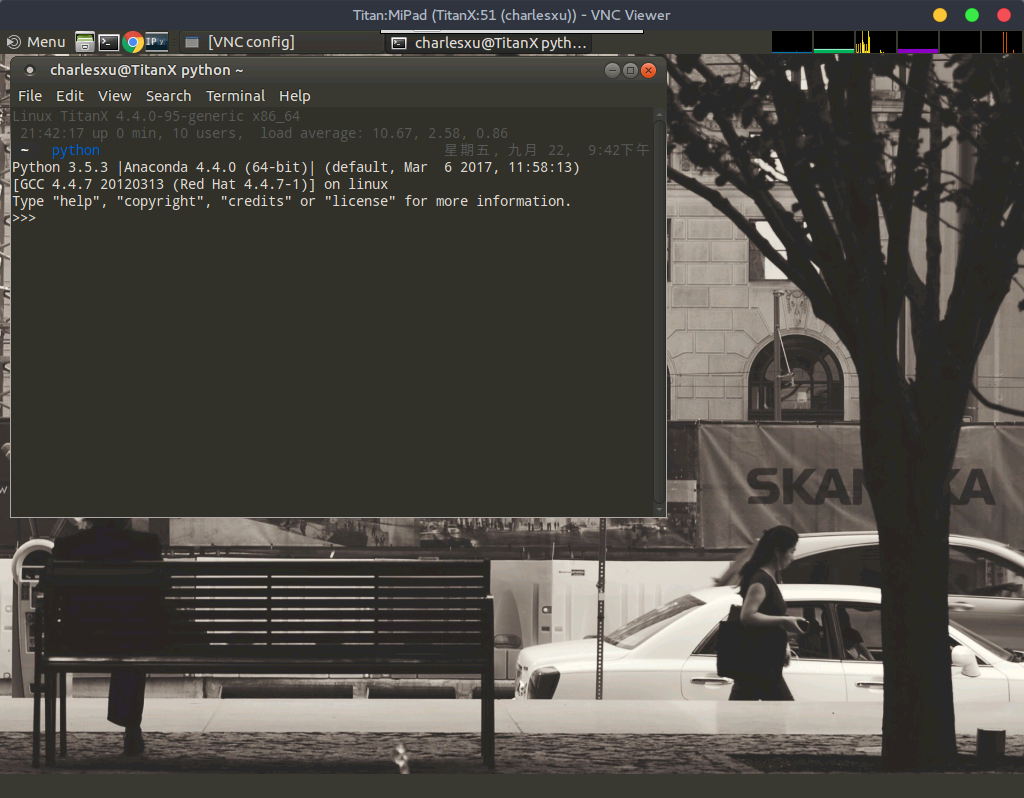
\includegraphics[width=0.8\hsize]{fig/os.jpg}
\caption{操作系统}
\label{os}
\end{figure}






\end{document}
